\documentclass[pdflatex,sn-mathphys-num]{sn-jnl}

\usepackage{graphicx}
\usepackage{multirow}
\usepackage{amsmath,amssymb,amsfonts}
\usepackage{amsthm}
\usepackage{mathrsfs}
\usepackage[title]{appendix}
\usepackage{xcolor}
\usepackage{colortbl}
\usepackage{textcomp}
\usepackage{manyfoot}
\usepackage{booktabs}
\usepackage{algorithm}
\usepackage{algorithmicx}
\usepackage{algpseudocode}
\usepackage{listings}
\usepackage{amsmath}
\usepackage{manyfoot}
\usepackage{mathrsfs}
\usepackage{algorithm}
\usepackage{algorithmicx}
\usepackage{algpseudocode}
\usepackage{listings}
\usepackage{booktabs}
\usepackage{multirow}
\usepackage{tikz}
\usetikzlibrary{shapes,arrows,positioning,calc,fit,backgrounds}
\usepackage{subcaption}
\usepackage{fontawesome5}
\usepackage{xspace}

\newcommand{\emAnger}{Anger\xspace}
\newcommand{\emEncouragement}{Encouragement\xspace}
\newcommand{\emJoy}{Joy\xspace}
\newcommand{\emGratitude}{Gratitude\xspace}
\newcommand{\Eone}{\colorbox{gray!15}{E1}\xspace}
\newcommand{\Etwo}{\colorbox{gray!30}{E2}\xspace}

\definecolor{cadmiumgreen}{rgb}{0.0, 0.42, 0.24}
\newcommand{\gray}[1]{{\color{gray}#1}}
\newcommand{\blue}[1]{{\color{blue}#1}}
\newcommand{\cadmiumgreen}[1]{{\color{cadmiumgreen}#1}}
\newcommand{\foo}{\hspace{1em}}


\theoremstyle{thmstyleone}
\newtheorem{theorem}{Theorem}
\newtheorem{proposition}[theorem]{Proposition}%
\theoremstyle{thmstyletwo}
\newtheorem{example}{Example}
\newtheorem{remark}{Remark}
\theoremstyle{thmstylethree}
\newtheorem{definition}{Definition}
\raggedbottom


\begin{document}

\title[]{Emotion Fidelity of AI-generated Human Avatars: Evaluation and Societal Impact}

%\author*[1]{\fnm{Alan} \sur{Guedes}}\email{a.guedes@reading.ac.uk}
%\affil[1]{\orgdiv{Department of Computer Science}, \orgname{University of Reading}, \orgaddress{\city{Reading}, \country{United Kingdom}}}
\author*[1]{\fnm{Anonymous} \sur{Author(s)}}\email{anonymous@example.com}
\affil[1]{\orgdiv{Department of Anonymous}, \orgname{Anonymous Institution}, \orgaddress{\city{Anonymous}, \country{Anonymous}}}

\abstract{ This paper presents a multi-disciplinary evaluation of emotional resonance and fidelity in videos generated by state-of-the-art Generative Artificial Intelligence (GenAI) models. Through a structured focus group session with film industry researchers, we assess the performance of Wan2.1, Hunyuan-Video, and Runway across text-to-video and audio-driven generation tasks. While current generative architectures achieve high visual quality, we identify significant limitations in their capacity to express subtle, complex human emotions. We examine these constraints, mapping the evolution of recent models and detailing the specific emotional expression deficits observed during user trials. We contextualize these results within the broader discussion of the responsible use of AI in art creation and archival practice, proposing frameworks that prioritize human artistic agency.}

\keywords{Generative AI, Humans Avatars, Video Synthesis}

\maketitle

\section{Introduction}\label{sec1}
The rapid advancement of Generative Artificial Intelligence (GenAI) has introduced a paradigm shift in visual media production, enabling the synthetic creation of photorealistic digital humans from text descriptions or audio recordings. In creative workflows, particularly within film and television, these models promise to streamline pre-visualization, character generation, and post-production effects. However, their integration into high-end cinematic production is bottlenecked by their struggle to convey subtle, complex, and psychologically coherent human emotions. While traditional computer-generated imagery (CGI) utilizes keyframing or motion capture to carefully map facial geometries to expressive states, GenAI models synthesize animation dynamically in a latent space, often overlooking the anatomical and psychological nuances of acting. This raises two central research questions: (RQ1) \textit{To what extent can generative models satisfy the expected somatic aspects of emotional performance when evaluated across key qualitative dimensions (Aesthetic Quality, Expression Realism, Emotional Intensity, and Temporal Coherence)?} and (RQ2) \textit{How do open-source, auditable architectures compare to proprietary models in terms of expressive fidelity and model inspectability?}

Through a structured focus group session conducted with film and television academics and student researchers at [Anonymized University]\footnote{\url{https://magenta-crepe-43d98a.netlify.app}}, we perform a qualitative evaluation of state-of-the-art open-source and commercial video generation models. We assess their performance across text-to-video (T2V) and audio-driven video synthesis pipelines, identifying structural limitations such as the uncanny valley effect, physical warping, and cross-modal disconnections. By highlighting these limitations, we argue for a more responsible, human-centric design of generative tools that respects acting heritage and supports rather than replaces creative human agency.

The primary contributions of this work are threefold. First, we provide a multi-disciplinary qualitative evaluation of state-of-the-art GenAI models (Wan 2.1, Hunyuan-Video, and Runway) in text-to-video and audio-driven contexts, highlighting critical somatic limitations such as the Duchenne smile deficit and cross-modal emotional disconnections. Second, we propose an evaluation framework structured around four qualitative dimensions (Aesthetic Quality, Expression Realism, Emotional Intensity, and Temporal Coherence) to assess performance depth, establishing this qualitative dimensions schema as a key contribution of this paper. Third, we address the ethical, labor, and legal landscapes surrounding digital human cloning, analyzing contract patterns and proposing statutory reforms for likeness protection.

The remainder of this paper is structured as follows. Section~\ref{sec:background} outlines the transition from manual 3D CGI to generative networks. Section~\ref{sec3} details our evaluation methodology, results, and discussion. Section~\ref{sec5:societal} addresses the societal, policy, and legal dimensions of digital likeness. Finally, Section~\ref{sec6} concludes the paper.

\section{Background}\label{sec:background}

\begin{table}[ht]
\caption{Historical timeline humans avatar generation methods.}\label{tab:evolution_timeline}
\begin{tabular}{l | @{\foo} p{10.5cm}}
    1978 & Ekman and Friesen publish the Facial Action Coding System (FACS)~\cite{ekman1978facial} \\
    1990s--2010s & Manual 3D CGI rigging and blendshape animation become movie industry standards \\
    2014 & Goodfellow et al. propose Generative Adversarial Networks (GANs)~\cite{goodfellow2014generative} \\
    2019 & Karras et al. introduce StyleGAN for high-fidelity static face synthesis~\cite{karras2019style} \\
    2020--2022 & Early video GANs (e.g., MoCoGAN) attempt video synthesis, but with low resolution  \\
    2022 & Rombach et al. introduce Latent Diffusion Models (LDMs)~\cite{rombach2022high} \\
    2023 & Stable Video Diffusion and Runway Gen-2 scale video generation, suffer from prompt drift and warping \\
    2023 & Peebles and Xie propose Diffusion Transformers (DiTs)~\cite{peebles2023scalable} \\
    2024 & Lipman et al. introduce Flow Matching for straight-path modeling~\cite{lipman2022flow} \\
         & Runway Gen-3 Alpha and Hunyuan-Video integrate DiTs for highly stable character generation~\cite{hunyuan2024video,runway2024gen3} \\
    2025 & Wan 2.1 open-source model released with spatial-temporal patch scaling~\cite{wan2025wan21} \\
\end{tabular}
\end{table}

The historical timeline presented in Table~\ref{tab:evolution_timeline} charts the transition from anatomical classification systems to data-driven statistical models for character synthesis. This trajectory began with the formulation of the Facial Action Coding System (FACS) in 1978, which established the anatomical foundation for facial animation. For decades, manual 3D computer-generated imagery (CGI) blendshape rigging remained the industry standard, offering absolute artistic control at the cost of high manual labor. The advent of deep learning in 2014 initiated a shift toward generative modeling. Generative Adversarial Networks (GANs) and StyleGAN enabled high-fidelity static face synthesis, while Latent Diffusion Models (LDMs) later solved spatial resolution issues. Most recently, Diffusion Transformers (DiTs) and Flow Matching have emerged as the leading paradigms, enabling highly stable temporal coherence in open-source models like Wan 2.1 and Hunyuan-Video. The following subsections will explore these primary paradigms in detail, focusing first on manual 3D CGI and subsequently on GenAI methods for human character generation.

\subsection{Manual 3D CGI video generation}\label{sec:manual_3d}


Historically, digital character creation relied on traditional computer-generated imagery (CGI), requiring specialized digital artists to manually keyframe blendshapes or record a performer's physical movements using complex optical motion capture (MoCap) rigs. While this classic production workflow guarantees absolute artistic control, precise frame-by-frame directing, and perfect temporal consistency, it remains highly labor-intensive, costly, and accessible only to high-budget major studios. Furthermore, the long-term preservation and digital archiving of these complex character assets present major format compatibility and software dependency challenges, as proprietary rigs and meshes quickly become obsolete. Traditional CGI facial animation is grounded in the Facial Action Coding System (FACS), developed by Paul Ekman and Wallace Friesen~\cite{ekman1978facial}. FACS taxonomizes human facial movements into individual Action Units (AUs), which correspond to the contraction of specific facial muscles. In professional 3D pipelines, a character rig is constructed with dozens of blendshapes (geometric target shapes) representing these AUs. By animating the activation levels of these blendshapes over time—either manually or by mapping motion capture data—animators can construct highly realistic, anatomically correct expressions. While FACS-based rigs provide complete control, they require an expert understanding of anatomy and hundreds of hours of manual tweaking. If an animator fails to balance the activation of key AUs (for example, activating the zygomaticus major for a smile without the orbicularis oculi), the expression loses its credibility.

\textbf{Motion Capture and Retargeting.} In modern motion capture pipelines, a performer wears a head-mounted camera (HMC) system equipped with high-speed cameras and infra-red or visible light tracking systems. The system tracks the 3D trajectories of dozens of retroreflective markers or painted tracking dots placed at key anatomical landmarks on the actor's face. The raw 3D marker coordinates must be mapped to the character's blendshape rigs through a process called motion retargeting. This requires solving a non-linear optimization problem at each frame to find the set of weights that minimizes the geometric distance between the performer's marker configuration and the character's mesh deformation, incorporating a regularization term to prevent sudden, erratic weight transitions (jitter) and enforce anatomically plausible weight configurations. Despite advanced optimization algorithms, the retargeted weights always require manual cleanup by digital animators to correct for marker sliding, occlusion, and differences in facial proportions between the actor and the digital character, adding substantial cost and time to the production pipeline.

\subsection{AI-based Human Video Synthesis}\label{sec2}
The transition from physical performance to digital character synthesis has occurred in distinct waves, moving from rigid geometric control to dynamic statistical estimation. Prominent examples of these technologies, such as the viral Tom Cruise TikTok deepfakes~\cite{tomcruisedeepfake} and the Jordan Peele/BuzzFeed Obama deepfake address~\cite{obamadeepfake} (shown in Figure~\ref{fig:deepfakes}), have brought the capability and societal impact of synthetic avatars into public awareness\footnote{\url{http://alanlivio.github.io/paper-eval-genai-movie-characters}}.

\begin{figure*}[ht!]
  \centering
  \begin{subfigure}[b]{0.31\textwidth}
    \centering
    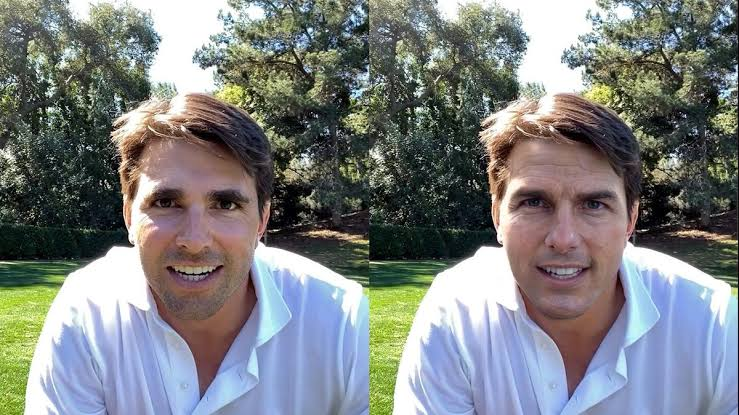
\includegraphics[width=\linewidth,height=2cm]{assets/tom-cruise.png}\\[3pt]
    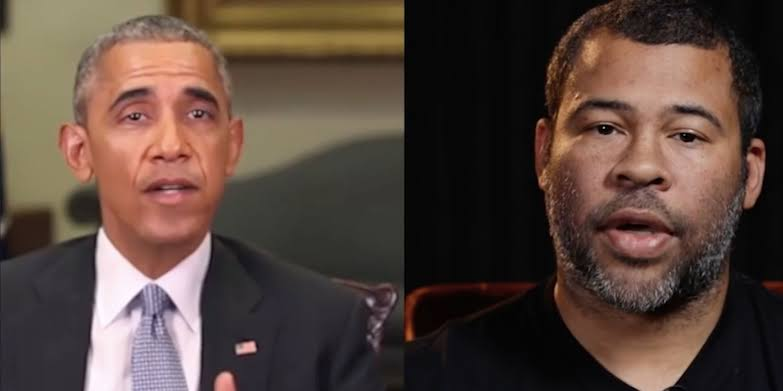
\includegraphics[width=\linewidth,height=2cm]{assets/obama.png}
    \caption{Viral deepfakes (Tom Cruise \cite{tomcruisedeepfake}, Obama \cite{obamadeepfake}).}
    \label{fig:deepfakes}
  \end{subfigure}
  \hfill
  \begin{subfigure}[b]{0.31\textwidth}
    \centering
    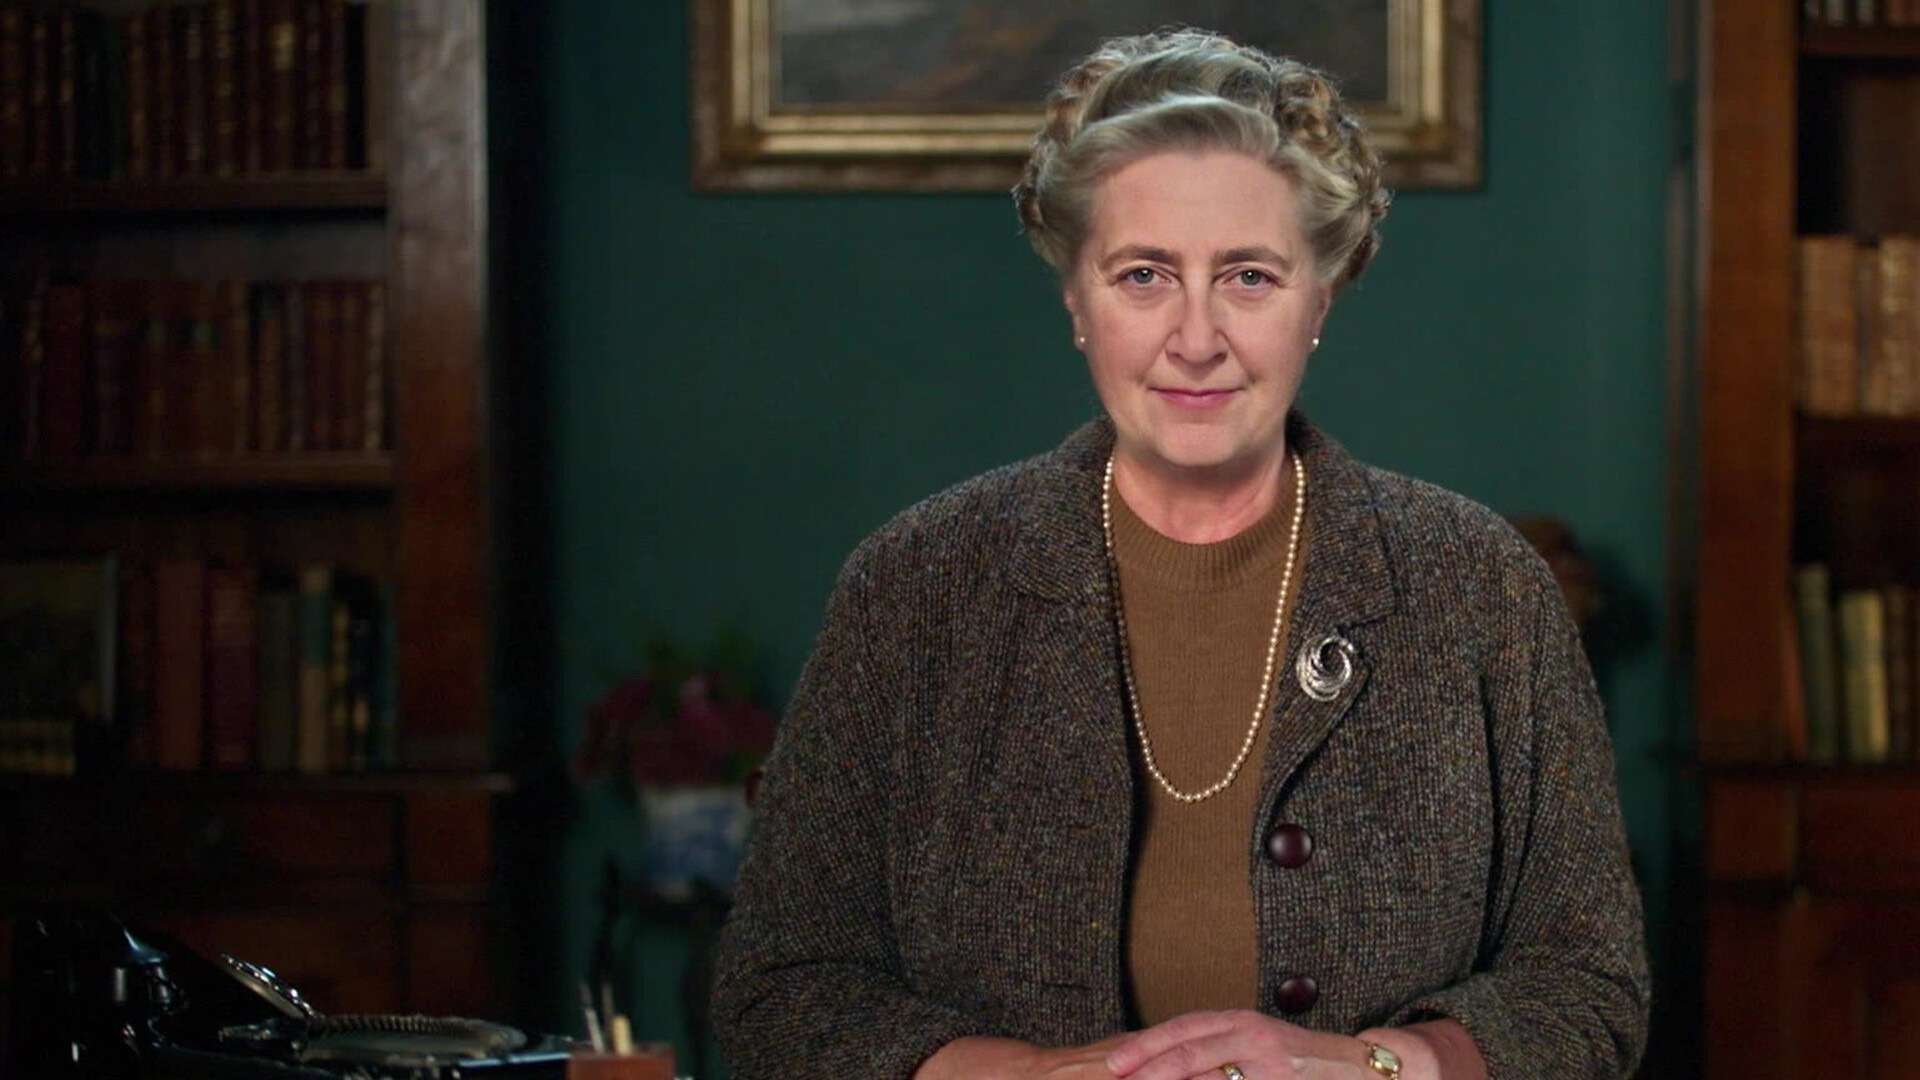
\includegraphics[width=\linewidth,height=2cm]{assets/agatha.png}\\[3pt]
    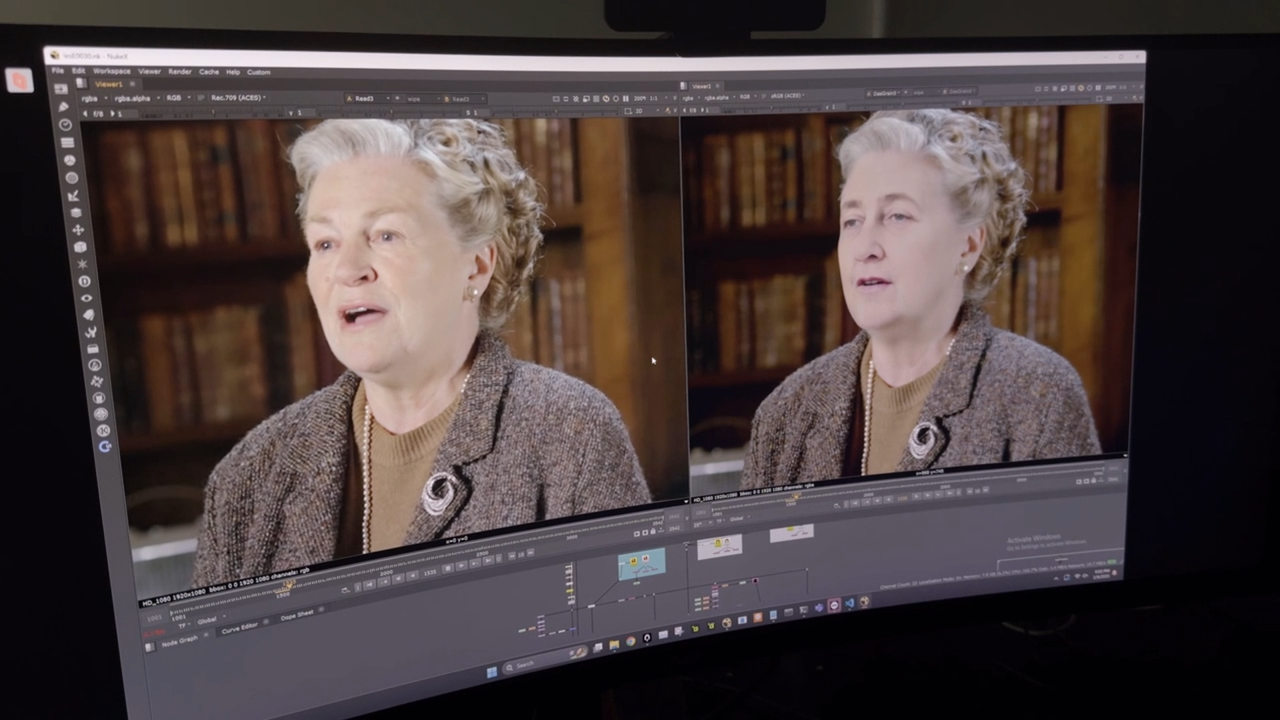
\includegraphics[width=\linewidth,height=2cm]{assets/agatha2.png}
    \caption{BBC Agatha Christie writing course \cite{bbcmaestroagatha}.}
    \label{fig:agatha}
  \end{subfigure}
  \hfill
  \begin{subfigure}[b]{0.31\textwidth}
    \centering
    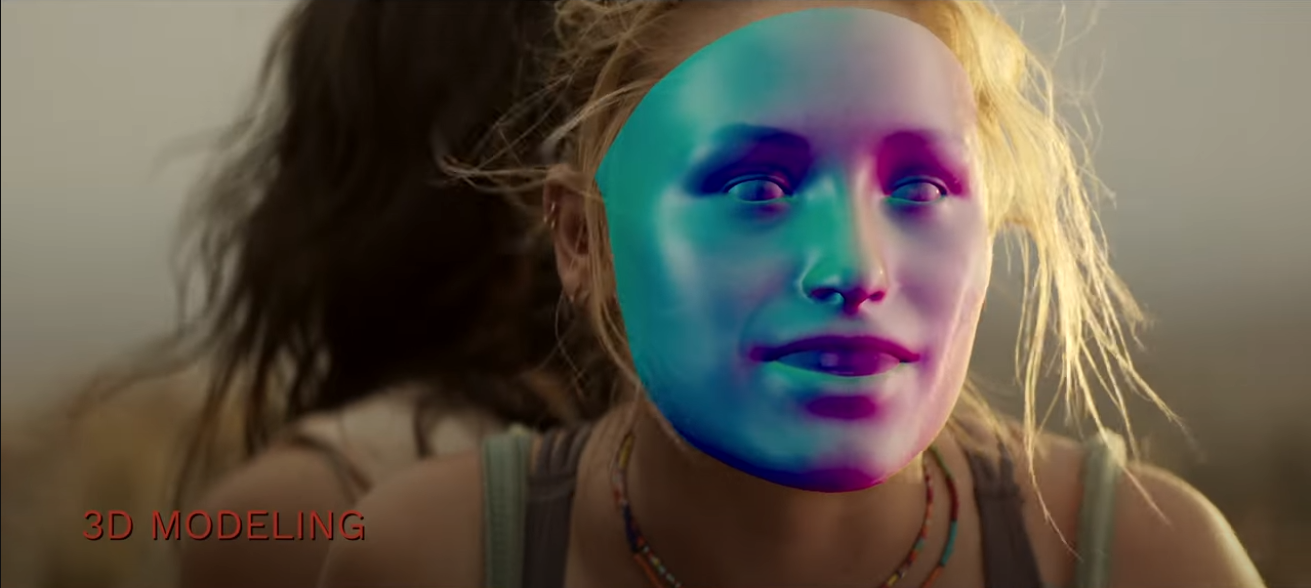
\includegraphics[width=\linewidth,height=2cm]{assets/replace1.png}\\[3pt]
    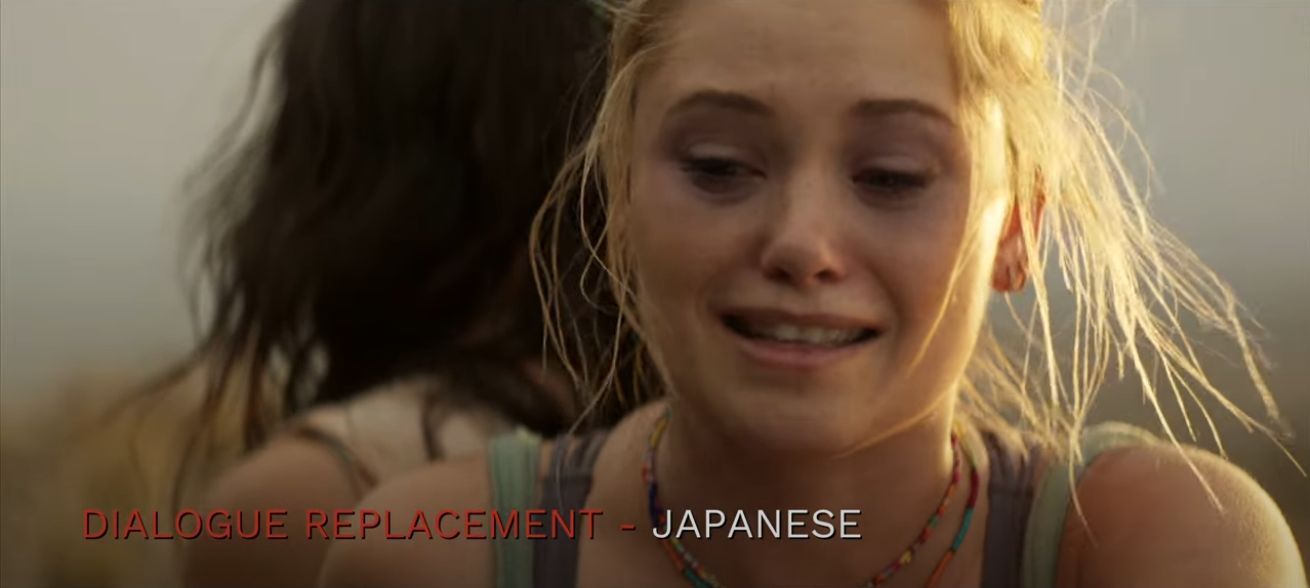
\includegraphics[width=\linewidth,height=2cm]{assets/replace2.png}
    \caption{Movie industry dialogue replacement \cite{truesyncdialogue}.}
    \label{fig:replace}
  \end{subfigure}
  \caption{Examples of generative tools and synthetic avatars: (a) viral face-swapping deepfakes, (b) automated scriptwriting and content generation, and (c) dialogue replacement.}
  \label{fig:background_overview}
\end{figure*}

\textbf{Early GAN and LDM Frameworks.} Early approaches utilized Generative Adversarial Networks (GANs)~\cite{goodfellow2014generative}, such as StyleGAN~\cite{karras2019style}, to generate high-fidelity static faces. Extending them to video required architectures like VideoGAN or MoCoGAN, which split latent spaces into content (identity) and motion vectors. These early video GANs suffered from low resolution, "mode collapse," and massive temporal drift. The subsequent introduction of Latent Diffusion Models (LDMs)~\cite{rombach2022high} solved many resolution challenges by executing the diffusion process in a compressed, low-dimensional latent space, enabling applications like content generation (Figure~\ref{fig:agatha}). However, early models like Runway Gen-2 still exhibited significant prompt drift, physical clipping under movement, and a lack of three-dimensional structural consistency, hindering their application in precise film dialogue replacement (Figure~\ref{fig:replace}).

\textbf{Diffusion Transformers.} Modern video generation has transitioned to data-driven statistical scaling, shifting the spatial backbone of video models from U-Nets to Diffusion Transformers (DiTs)~\cite{peebles2023scalable}. The video latent volume is partitioned into non-overlapping 3D spatial-temporal patches, projected as token sequences, and combined with 3D positional encodings (e.g., RoPE) to capture global spatial and temporal dependencies through self-attention layers. Conditioning inputs, such as text prompts (via T5) or speech audio (via Wav2Vec), are injected via cross-attention. To optimize the generation process, these pipelines implement Flow Matching~\cite{lipman2022flow}, which defines a deterministic vector field to generate straight-path trajectories in the latent space, allowing standard numerical ODE solvers to synthesize stable videos in only 20--30 steps. Although this transformer-based latent mapping scales effectively in models like Hunyuan-Video~\cite{hunyuan2024video}, Wan 2.1~\cite{wan2025wan21}, and Runway Gen-3 Alpha~\cite{runway2024gen3}, it remains a statistical estimator. Lacking biophysical, skeletal, or anatomical constraints, it relies purely on statistical correlations, resulting in the emotional and physical performance distortions observed in our evaluations.

\begin{figure}[ht!]
  \centering
  \resizebox{\textwidth}{!}{%
  \begin{tikzpicture}[
    node distance=1.2cm and 1.5cm,
    block/.style={draw, fill=gray!15, rectangle, minimum height=2.2em, minimum width=7.5em, rounded corners, align=center, font=\small},
    input/.style={draw, fill=white, rectangle, minimum height=2.2em, minimum width=7em, align=center, font=\small},
    process/.style={draw, fill=gray!30, rectangle, minimum height=2.2em, minimum width=8.5em, rounded corners, align=center, font=\small},
    arrow/.style={draw, ->, >=stealth, thick}
  ]
    % Input nodes
    \node [input] (text) {\faKeyboard~Text Prompt};
    \node [input, below=0.8cm of text] (audio) {\faMusic~Audio Input};
    
    % Encoders
    \node [block, right=of text] (text_enc) {Text Encoder\\(e.g., T5)};
    \node [block, right=of audio] (audio_enc) {Audio Encoder\\(e.g., Wav2Vec)};
    
    % Fusion & Conditioning
    \node [process, right=1.2cm of $(text_enc.east)!0.5!(audio_enc.east)$] (conditioning) {Cross-Attention \&\\Conditioning Layer};
    
    % DiT Blocks
    \node [block, right=1.2cm of conditioning] (dit) {Diffusion Transformer\\(DiT) Blocks};
    
    % Output
    \node [input, right=of dit] (output) {\faVideo~Generated\\Video Output};
    
    % Draw arrows
    \draw [arrow] (text) -- (text_enc);
    \draw [arrow] (audio) -- (audio_enc);
    \draw [arrow] (text_enc.east) -- ++(0.4,0) |- (conditioning.west);
    \draw [arrow] (audio_enc.east) -- ++(0.4,0) |- (conditioning.west);
    \draw [arrow] (conditioning) -- (dit);
    \draw [arrow] (dit) -- (output);
    
  \end{tikzpicture}
  }
  \caption{Conditioning pathways in modern Diffusion Transformer (DiT) video generation architectures, supporting both text-only generation (top pipeline) and audio-guided generation (bottom pipeline) conditioning noisy video patches.}
  \label{fig:dit_architecture}
\end{figure}

\section{Evaluation of Emotional Fidelity in Human Avatars}\label{sec3}

\begin{figure}[ht!]
  \centering
  \resizebox{\textwidth}{!}{%
  \begin{tikzpicture}[
    node distance=1.5cm,
    block/.style={draw=black!70, fill=gray!10, rectangle, rounded corners, thick, align=center, inner sep=10pt, font=\small, minimum width=4cm, minimum height=1.5cm},
    input/.style={draw=black!40, fill=gray!2, dashed, rectangle, rounded corners, align=center, inner sep=6pt, font=\footnotesize, minimum width=3.5cm},
    arrow/.style={draw, ->, >=stealth, thick, black!70}
  ]
    \node [input] (audio) {\textbf{Audio Input}\\(e.g., J. Nicholson voice)};
    \node [input, below=0.4cm of audio] (ref) {\textbf{Reference Image}\\(e.g., J. Nicholson frame)};
    
    \node [block, right=1.2cm of audio, yshift=-0.5cm] (gen) {\textbf{Video Generation}\\(Wan 2.1 / Runway Gen-3)\\ \vspace{0.1cm} \faVideo};
    \node [block, right=of gen] (analysis) {\textbf{FTT Analysis}\\(E1/E2 Evaluation)\\ \vspace{0.1cm} \faUser\quad\faClipboardCheck};
    \node [block, right=of analysis] (summary) {\textbf{Feedback Summary}\\(Qualitative Dimensions)\\ \vspace{0.1cm} \faComments};
    
    \draw [arrow] (audio.east) -- ++(0.4,0) |- ([yshift=0.2cm]gen.west);
    \draw [arrow] (ref.east) -- ++(0.4,0) |- ([yshift=-0.2cm]gen.west);
    \draw [arrow] (gen) -- (analysis);
    \draw [arrow] (analysis) -- (summary);
  \end{tikzpicture}
  }
  \caption{Evaluation workflow framework showing three distinct blocks: Video Generation (receiving audio input and reference image), FTT Analysis, and Feedback Summary.}
  \label{fig:audio_generation_pipeline}
\end{figure}To evaluate how state-of-the-art generative models capture human emotion, we designed a structured focus group evaluation. This evaluation tracks the fidelity of synthetic avatars created from iconic movie scenes across different generation pipelines. We analyze the process of exporting generated video frames and managing key frames to assess motion consistency and temporal degradation. To address both RQ1 (emotional acting replication) and RQ2 (open-source vs. proprietary architectures), we designed our evaluation to directly contrast open-source, auditable models (Model A: Hunyuan-Video-Avatar / Wan 2.1) against black-box, proprietary pipelines (Model B: Runway). While proprietary models offer high visual resolution, their closed nature prevents auditing the training data or underlying alignment. Open-source models, on the other hand, permit inspecting their weights and intermediate latent layers, which is crucial for auditing representations of diverse somatic features and expressions. In the following subsections, we discuss the video generation process and the qualitative evaluation from industry experts.

\subsection{Video Generation}\label{subsec:video_generation}

To evaluate the current state of emotional performance in generative video, this study focuses on audio-driven facial synthesis, which represents a sub-field of video generation where speech audio animates a digital character. Early models like Wav2Lip utilized discriminators to enforce lip-sync accuracy, while models like SadTalker introduced facial landmark generators to simulate natural head motion and blinking. In contemporary pipelines, such as Hunyuan-Video-Avatar, speech audio is processed through audio encoders (like Wav2Vec) and mapped directly to spatial-temporal latent representations. While these models achieve highly accurate lip-syncing, they suffer from a severe "emotional disconnect." Because they map phonemes to lip movements, they fail to model the emotional state of the speaker. A trembling, tearful voice track will animate the lips to form the correct words, but the eyes, forehead, and cheeks will remain static and unexpressive.

All video generation and evaluation trials were executed using the ComfyUI platform on identical workstations equipped with AMD Ryzen 9 5900X processors, 64 GB of DDR4 RAM, and NVIDIA GeForce RTX 4090 GPUs (24 GB VRAM).

To empirically evaluate the emotional limitations of these architectures, we conducted a qualitative evaluation of audio-driven performance synthesis using four iconic scenes from classic cinema. These scenes were selected to cover a wide spectrum of emotional intensity and somatic complexity:

\begin{itemize}
    \item \textbf{\emAnger:} Jack Nicholson's courtroom monologue in \textit{A Few Good Men} (\url{https://www.youtube.com/watch?v=9FnO3igOkOk}). This scene was selected to evaluate explosive vocal projection, clenched jaw muscles, dynamic head movements, and facial micro-expressions of contempt under high-intensity rage.
    \item \textbf{\emEncouragement:} Sylvester Stallone's inspirational speech to his son in \textit{Rocky Balboa} (\url{https://www.youtube.com/watch?v=D_Vg4uyYwEk}). This scene was selected to evaluate the model's ability to sync speech audio under lower vocal frequencies while maintaining consistent jaw articulation and concentrated, emotionally charged eye contact.
    \item \textbf{\emJoy:} Robin Williams' class scenes in \textit{Dead Poets Society} (\url{https://www.youtube.com/watch?v=gS7tJ2P1L6c}). This scene was selected to evaluate how models capture warm, natural transitions of genuine joy, facial animation during smiles, and relaxed eye involvement.
    \item \textbf{\emGratitude:} Robin Williams and Matt Damon's counseling scene ("It's not your fault") in \textit{Good Will Hunting} (\url{https://www.youtube.com/watch?v=qM-gZezn1-Y}). This scene was selected to evaluate the expression of vulnerability, subtle eye movements, vocal trembling, and the complex somatic delivery of gratitude and cathartic relief.
\end{itemize}

Character screenshots and the original actor voice tracks were extracted from these scenes and processed through Model\_A (Hunyuan-Video-Avatar) and Model\_B (Runway) to generate corresponding synthetic characters.

\subsection{Qualitative Evaluation}\label{subsec:qualitative_evaluation}

A focus group consisting of 2 academics with expertise in actor training, cinematic performance analysis, or synthetic media production qualitatively compared the generated characters directly to the baseline actor performances, focusing on visual aesthetics, expression realism, emotional intensity, and temporal stability. To analyze the qualitative nuances across each evaluated emotion, we examine the feedback, observations, and key frames compiled in the expert columns of Table~\ref{tab:expert_feedback_anger_enc} and Table~\ref{tab:expert_feedback_joy_grat}, with detailed video outputs and comparative demos hosted on the companion project webpage\footnote{\url{https://magenta-crepe-43d98a.netlify.app}}:
\begin{itemize}
    \item \textbf{\emAnger:} In the Jack Nicholson courtroom monologue sequence, \Eone noted a stark contrast between Runway's high visual resolution and its flat, vacant expression delivery (the "blank stare"), observing that the eyes did not narrow and the brow remained un-furrowed despite the aggressive prompt. \Etwo agreed that Runway's anger felt superficial, resembling a neutral mask with an open mouth. For Wan 2.1, both experts highlighted severe face warping and distortion, with \Eone observing that the teeth appeared to float independently, and \Etwo noting that the animation broke the suspension of disbelief due to temporal inconsistencies and a jittery, disjointed head motion.
    \item \textbf{\emEncouragement:} For the Sylvester Stallone motivational speech, \Eone observed that Runway maintained a steady head pose but the eyes remained dead and unresponsive, with the lips moving but the rest of the face failing to participate. \Etwo characterized this delivery as flat and robotic, pointing out the disconnect where the tone of voice suggests passion but the face suggests indifference. For Wan 2.1, \Eone noted the accurate lip-syncing but highlighted a failure to connect vocal intensity with upper facial expressions, while \Etwo pointed out cheek distortions and sliding skin textures.
    \item \textbf{\emJoy:} In the Robin Williams classroom scene, \Eone noted that Runway's smile felt fake or "plastic," failing to engage the eyes (Duchenne smile deficit). \Etwo characterized Runway's output as an animated stock photo lacking warm, natural transitions. For Wan 2.1, \Eone observed that the model struggled to keep facial structure stable while smiling, leading to melting or warping around the nose and mouth, while \Etwo noted poor temporal coherence with teeth merging into a solid block.
    \item \textbf{\emGratitude:} For the counseling scene, the cross-modal mismatch was highly pronounced. \Eone observed that Runway's emotional tone was lost, resulting in a blank look rather than appreciation, and \Etwo noted that the character lacked micro-expressions of vulnerability, failing to project any internal psychological state. In the Wan 2.1 version, \Eone observed that while the vocal track was trembling and emotional, the eyes remained vacant, and \Etwo confirmed that the eye area remained static while the mouth shape changed.
\end{itemize}

\begin{table*}[ht]
\centering
\caption{Expert Feedback on \emAnger and \emEncouragement Expressions}
\label{tab:expert_feedback_anger_enc}
\makebox[\textwidth][c]{%
\begin{tabular}{p{2.8cm}p{2.8cm}>{\columncolor{gray!10}}p{5.0cm}>{\columncolor{gray!20}}p{5.0cm}}
\toprule
\textbf{Input} & \textbf{Output} & \textbf{E1} & \textbf{E2} \\
\midrule
{\centering
\raisebox{-.5\height}{
\includegraphics[width=2.5cm]{assets/actor_anger.png}} \par Anger scene \par\vspace{0.3cm}
\raisebox{-.5\height}{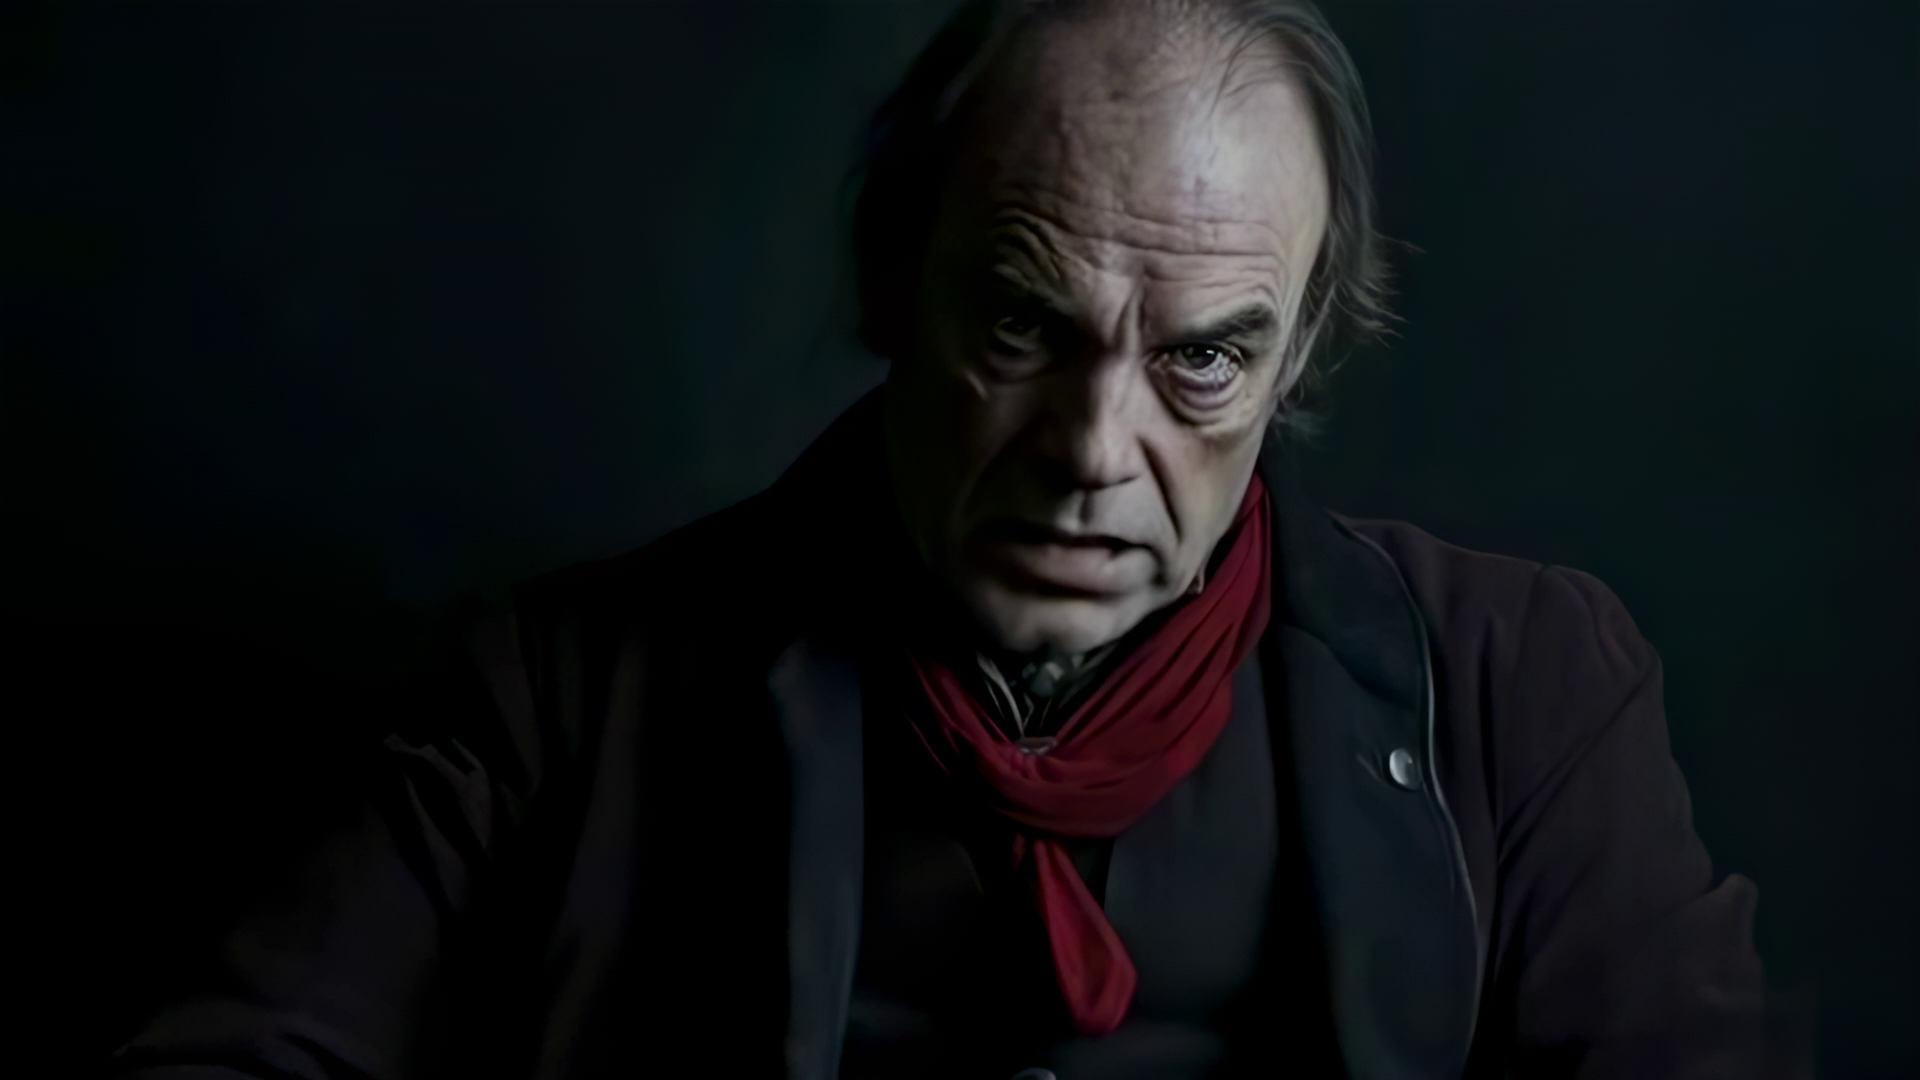
\includegraphics[width=2.5cm]{assets/ref_anger.png}} \par Reference image \par}
&
{\centering
\raisebox{-.5\height}{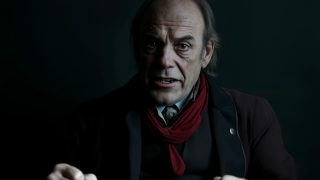
\includegraphics[width=2.5cm]{assets/Runway_anger.png}} \par A) Runway \par\vspace{0.3cm}
\raisebox{-.5\height}{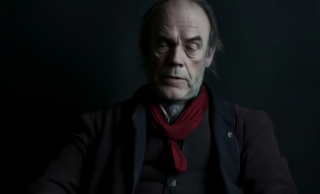
\includegraphics[width=2.5cm]{assets/Wan21_anger.png}} \par B) Wan 2.1 \par}
&
\textbf{A) Runway:} \textit{High visual quality and resolution, but the character has a relatively static face with a blank stare, lacking emotional micro-expressions. The eyes do not narrow and the brow remains un-furrowed despite the aggressive prompt.} \par\vspace{0.4cm}
\textbf{B) Wan 2.1:} \textit{Severe face warping and distortion under high-intensity emotion. The jaw and mouth area show artifacting, and the teeth appear to float independently.}
&
\textbf{A) Runway:} \textit{The anger feels superficial; the character's facial muscles do not contract realistically to match high-intensity rage. It looks like a neutral mask with an open mouth.} \par\vspace{0.4cm}
\textbf{B) Wan 2.1:} \textit{The animation breaks suspension of disbelief due to temporal inconsistencies and facial stretching. The head moves in a jittery, disjointed motion.} \\
\midrule
{\centering
\raisebox{-.5\height}{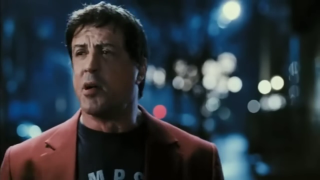
\includegraphics[width=2.5cm]{assets/actor_encouragement.png}} \par Encouragement scene \par\vspace{0.3cm}
\raisebox{-.5\height}{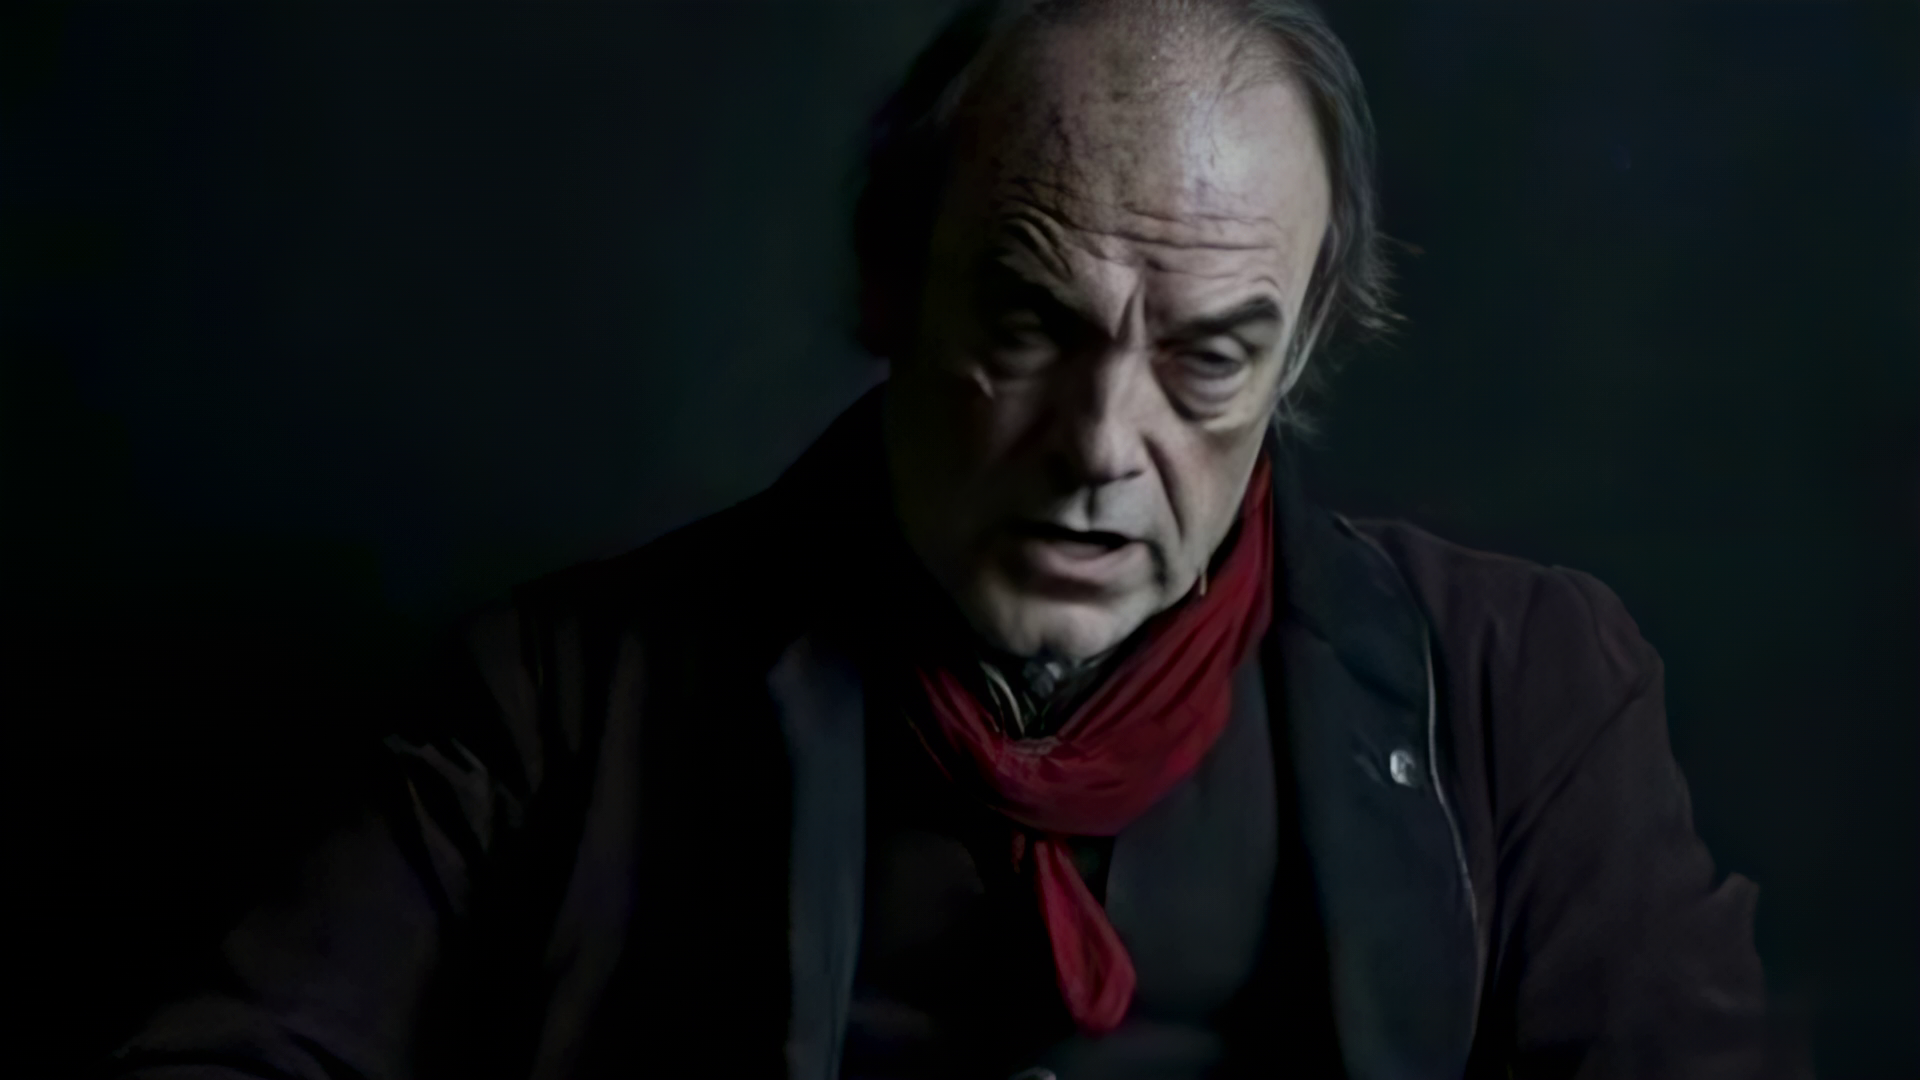
\includegraphics[width=2.5cm]{assets/ref_encouragement.png}} \par Reference image \par}
&
{\centering
\raisebox{-.5\height}{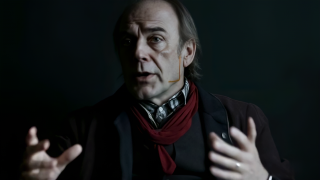
\includegraphics[width=2.5cm]{assets/Runway_encouragement.png}} \par A) Runway \par\vspace{0.3cm}
\raisebox{-.5\height}{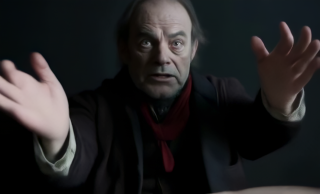
\includegraphics[width=2.5cm]{assets/Wan21_encouragement.png}} \par B) Wan 2.1 \par}
&
\textbf{A) Runway:} \textit{Steady head pose, but the eyes remain dead and unresponsive. The lips move to speak, but the rest of the face does not participate in the motivational delivery.} \par\vspace{0.4cm}
\textbf{B) Wan 2.1:} \textit{Accurate lip-syncing but fails to connect vocal intensity with upper facial expressions, resulting in a disconnected and confusing performance.}
&
\textbf{A) Runway:} \textit{The motivational expression is flat and robotic, lacking the nuance of a trained actor. The tone of voice suggests passion, but the face suggests indifference.} \par\vspace{0.4cm}
\textbf{B) Wan 2.1:} \textit{Distortions occur in the cheek area during larger head movements, with skin textures appearing to slide over the underlying bone structure.} \\
\bottomrule
\end{tabular}%
}
\end{table*}

\begin{table*}[ht]
\centering
\caption{Expert Feedback on \emJoy and \emGratitude Expressions}
\label{tab:expert_feedback_joy_grat}
\makebox[\textwidth][c]{%
\begin{tabular}{p{2.8cm}p{2.8cm}>{\columncolor{gray!10}}p{5.0cm}>{\columncolor{gray!20}}p{5.0cm}}
\toprule
\textbf{Input} & \textbf{Output} & \textbf{E1} & \textbf{E2} \\
\midrule
{\centering
\raisebox{-.5\height}{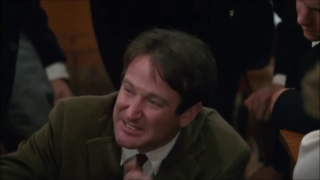
\includegraphics[width=2.5cm]{assets/actor_joy.png}} \par Joy scene \par\vspace{0.3cm}
\raisebox{-.5\height}{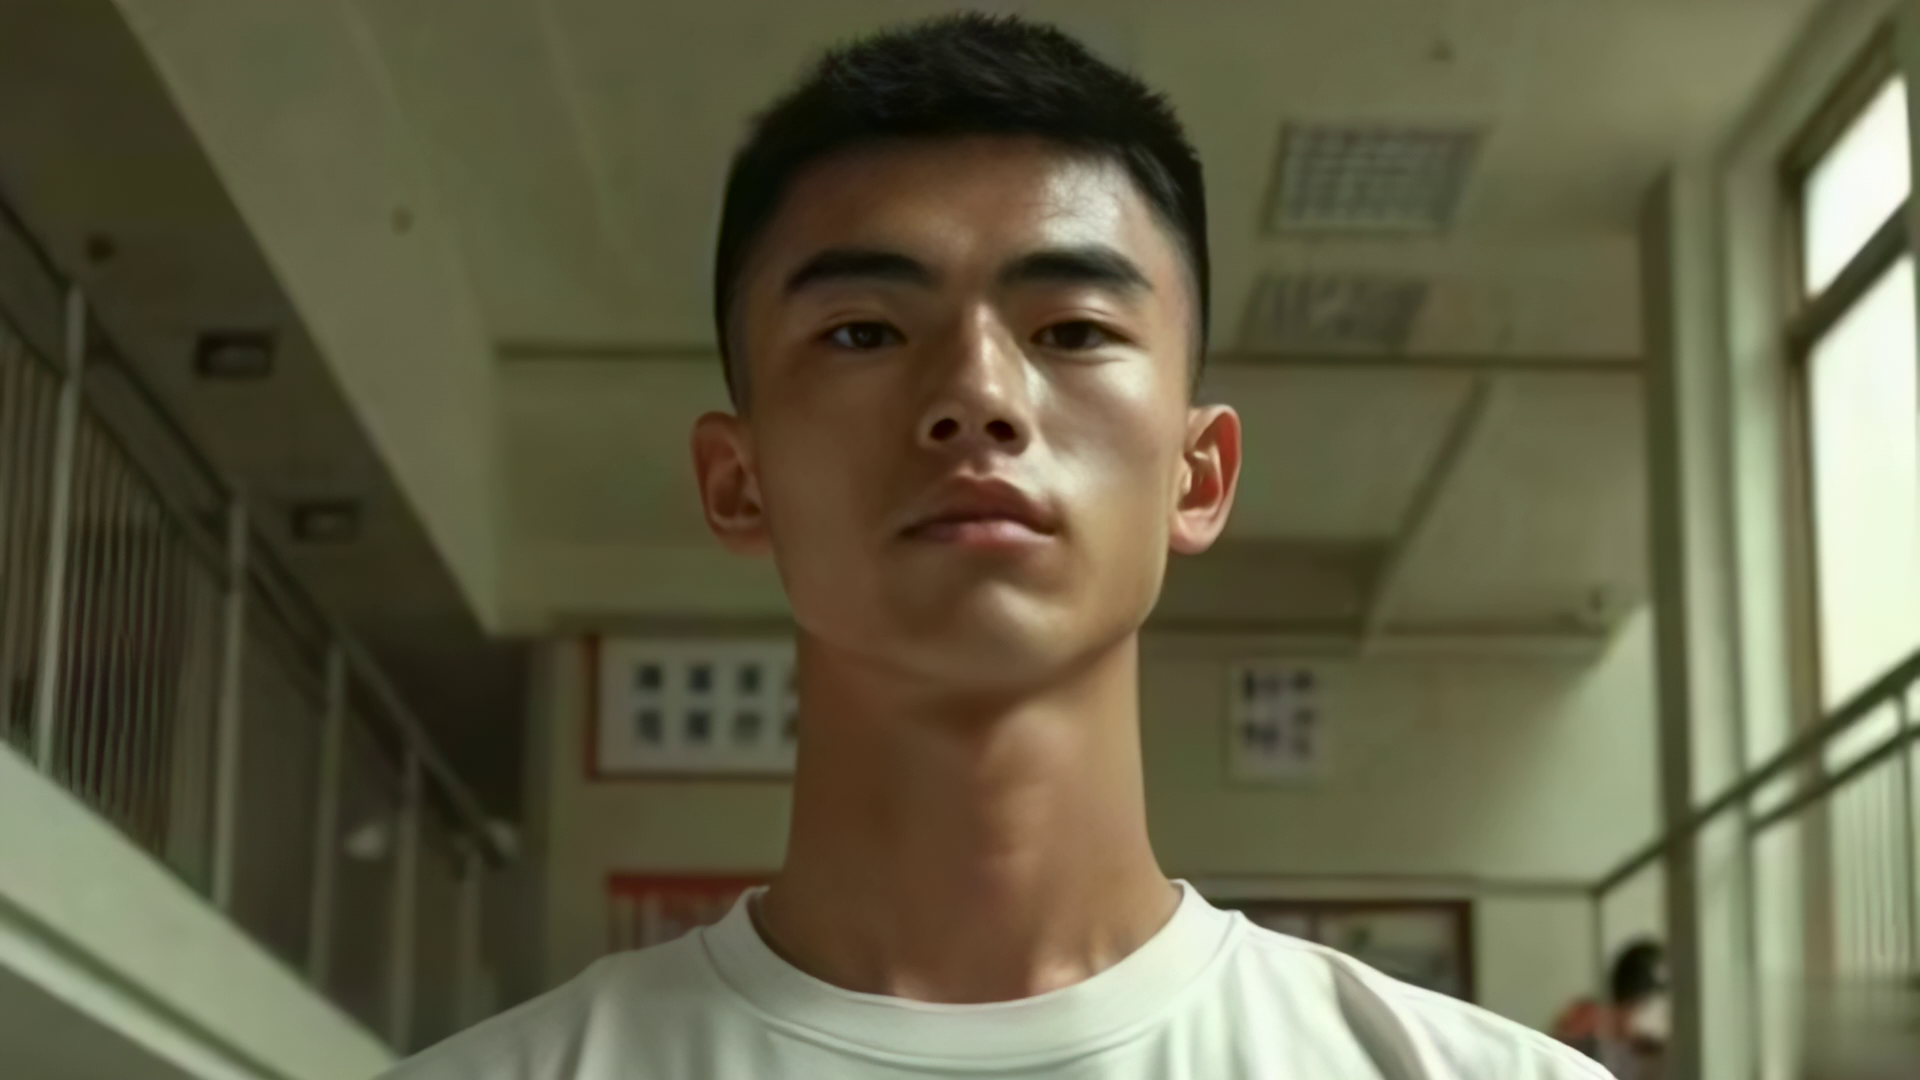
\includegraphics[width=2.5cm]{assets/ref_joy.png}} \par Reference image \par}
&
{\centering
\raisebox{-.5\height}{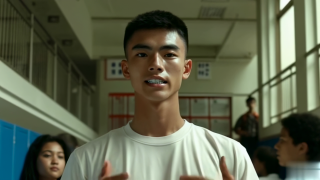
\includegraphics[width=2.5cm]{assets/Runway_joy.png}} \par A) Runway \par\vspace{0.3cm}
\raisebox{-.5\height}{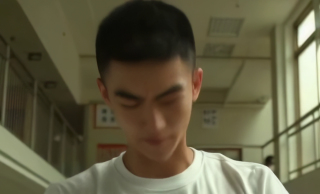
\includegraphics[width=2.5cm]{assets/Wan21_joy.png}} \par B) Wan 2.1 \par}
&
\textbf{A) Runway:} \textit{High aesthetic appeal, but the smile feels fake or ``plastic'', failing to engage the eyes (Duchenne smile deficit). The cheeks raise but the eyes do not crinkle.} \par\vspace{0.4cm}
\textbf{B) Wan 2.1:} \textit{Struggles to keep facial structure stable while smiling, leading to melting or warping around the nose and mouth.}
&
\textbf{A) Runway:} \textit{Looks like a stock photo animated; lacks the warm, natural transitions of genuine joy. The transitions between states are too linear and mechanical.} \par\vspace{0.4cm}
\textbf{B) Wan 2.1:} \textit{Poor temporal coherence around the teeth and lips. The teeth seem to merge into a solid white block during the smile.} \\
\midrule
{\centering
\raisebox{-.5\height}{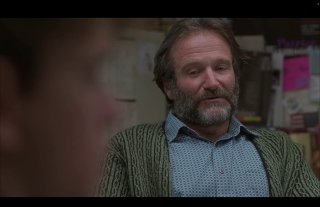
\includegraphics[width=2.5cm]{assets/actor_grateful.png}} \par Gratitude scene \par\vspace{0.3cm}
\raisebox{-.5\height}{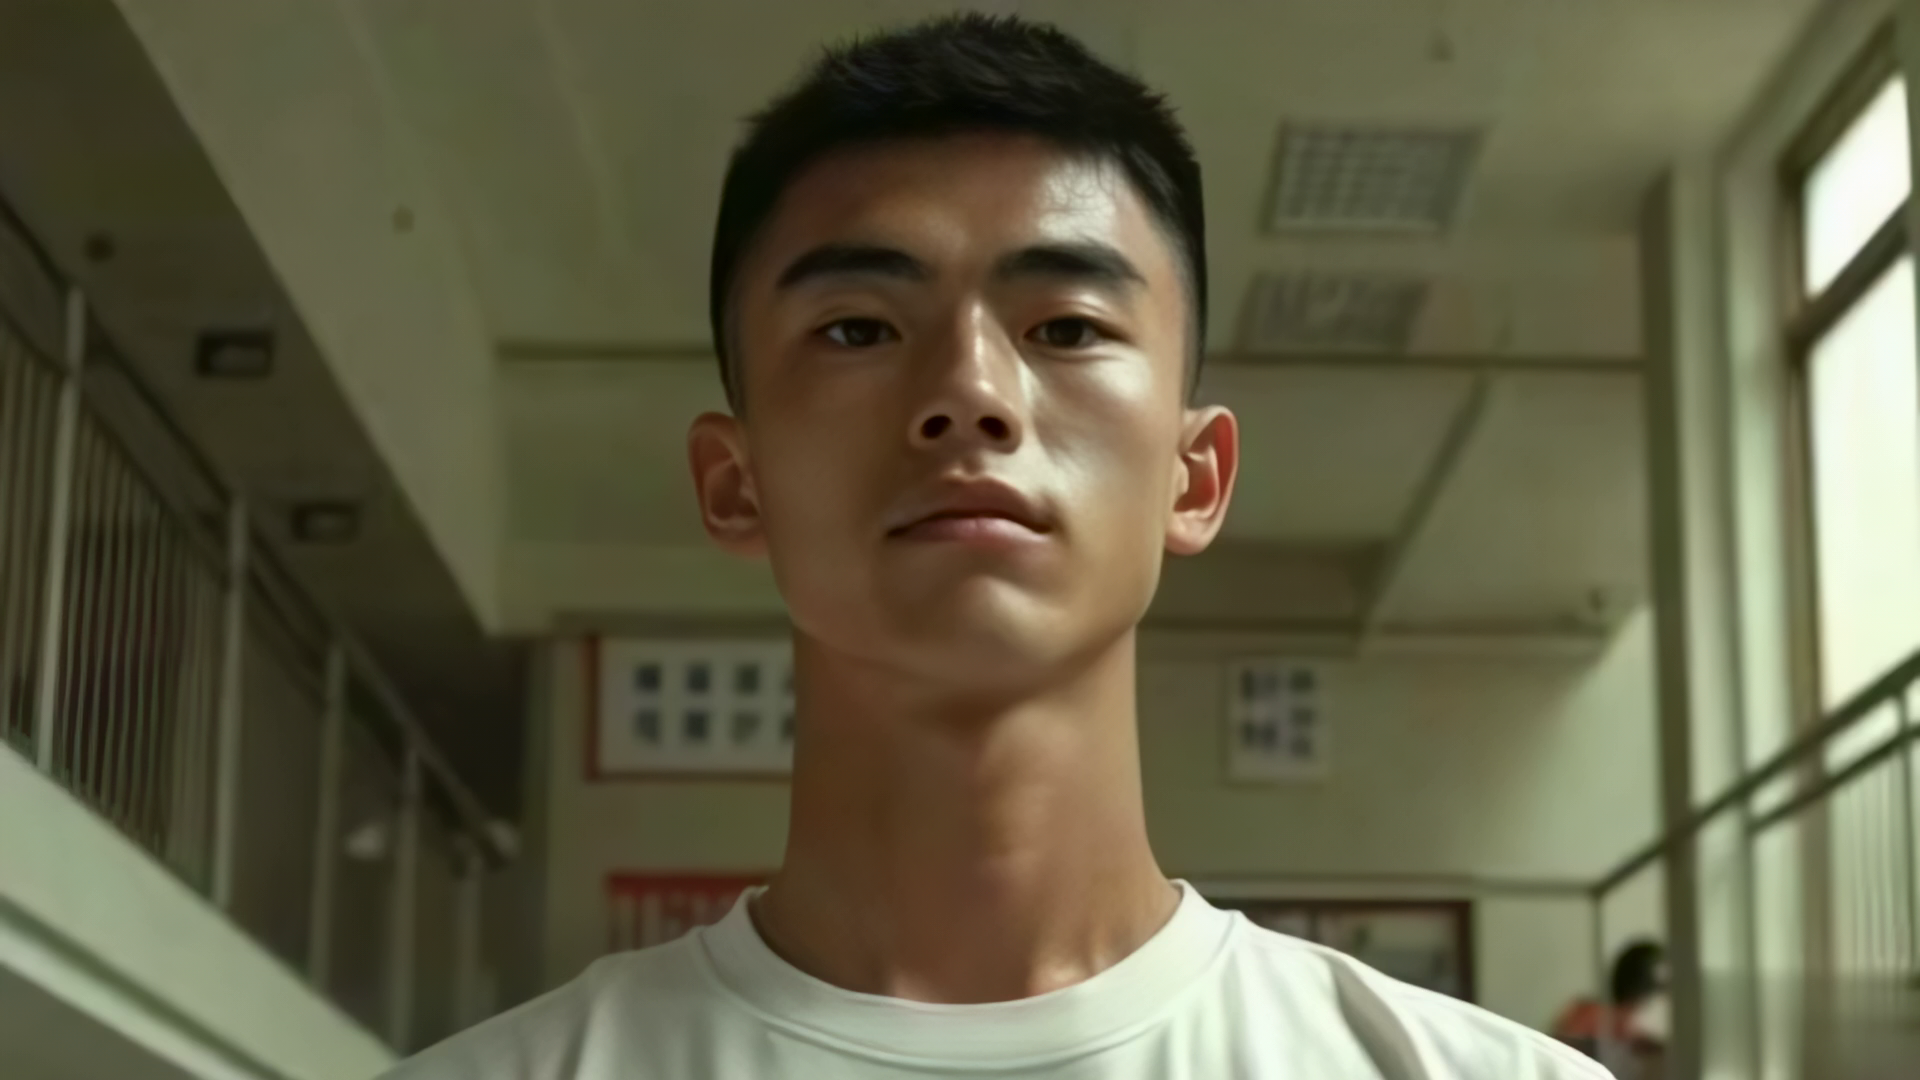
\includegraphics[width=2.5cm]{assets/ref_grateful.png}} \par Reference image \par}
&
{\centering
\raisebox{-.5\height}{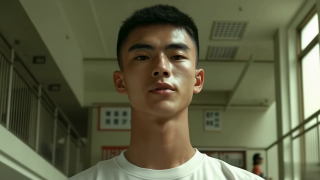
\includegraphics[width=2.5cm]{assets/Runway_grateful.png}} \par A) Runway \par\vspace{0.3cm}
\raisebox{-.5\height}{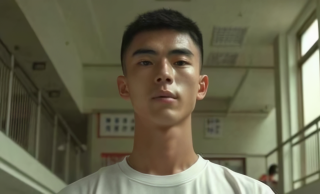
\includegraphics[width=2.5cm]{assets/Wan21_grateful.png}} \par B) Wan 2.1 \par}
&
\textbf{A) Runway:} \textit{The emotional tone is lost, resulting in a neutral or blank look rather than gratitude. The performance lacks the subtle facial softening that denotes appreciation.} \par\vspace{0.4cm}
\textbf{B) Wan 2.1:} \textit{Cross-modal mismatch; voice is trembling and emotional, but the eyes are completely vacant, showing no recognition of the weight of the moment.}
&
\textbf{A) Runway:} \textit{The character doesn't show the micro-expressions of vulnerability or emotion. It is too passive and fails to project any internal psychological state.} \par\vspace{0.4cm}
\textbf{B) Wan 2.1:} \textit{The model cannot animate subtle eye movements (like welling up) to match the audio. The eye area remains static while the mouth shape changes.} \\
\bottomrule
\end{tabular}%
}
\end{table*}

\textbf{Performance Fidelity and the Uncanny Valley.} A primary finding from our study is the deep divergence between aesthetic quality and emotional performance depth, which can be traced directly to the optimization techniques of modern video models. The implementation of Flow Matching~\cite{lipman2022flow} to define straight vector paths in the latent space is highly effective for reducing inference steps and ensuring high visual quality. However, this straight-path trajectory optimization suppresses the non-linear, high-frequency facial microkinesics required to convey genuine psychological states. For example, during the trials for the emotion of \emJoy, Runway Gen-3 generated a static, mouth-only smile that lacked the warm transitions of natural expression, which \Eone described as fake or "plastic," failing to engage the eyes (Duchenne smile deficit). Crucially, the model's linear latent path interpolation failed to animate the contraction of the orbicularis oculi muscles surrounding the eyes, which is the defining anatomical characteristic of a genuine Duchenne smile. This lack of organic coordination produces a mechanical and insincere appearance that \Etwo observed breaks the suspension of disbelief. In our text-to-video (T2V) trials, while Hunyuan-Video (Model B) attempted to introduce creative narrative elements, it struggled to animate a progressive emotional arc, instead rendering a series of disjointed frames. Similarly, in the football celebration scenario, the models' attempt to animate dynamic body movements resulted in severe jittering and identity drift, demonstrating that optimizing for visual aesthetics via linear flow matching does not translate into believable performance.

\textbf{Structural Limitations and Cross-Modal Disconnection.} High-intensity emotional prompts, such as Desperation or \emAnger, present a severe challenge to latent space representations. Because Diffusion Transformers (DiTs)~\cite{peebles2023scalable} partition video volumes into non-overlapping 3D spatial-temporal patches and project them as token sequences without underlying skeletal or anatomical priors, the models lack a structural constraint to maintain facial proportions under stress. Under these conditions, both Wan 2.1 and Hunyuan-Video suffered from significant geometric distortions and facial warping. To convey anger, the models stretched the facial tokens beyond biological limits, leading to unnatural jaw displacement, tooth clipping, and asymmetrical eye movement. \Eone observed that the teeth appeared to float independently, while \Etwo noted that the head moved in a jittery, disjointed motion. Rather than conveying a psychological state, the models distorted the character's geometry, pushing the synthetic actor deep into the uncanny valley. Furthermore, participants observed unexpected attribute shifts during these high-intensity prompts. Under the \emAnger prompt, Hunyuan-Video unilaterally altered the character's hair texture to an afro, illustrating how generative models default to stereotypic associations embedded in their training datasets. In audio-driven trials, the models frequently over-acted, producing exaggerated facial movements that fluctuated erratically between frozen states and hyper-dynamic distortions, highlighting the absence of underlying structural or skeletal rig constraints in standard diffusion architectures.


\subsection{Results Discussion}\label{sec5:technical}

In our audio-driven experiments, the lack of phase and emotional alignment between vocal cues and facial expressions was highly pronounced. For instance, in the *Good Will Hunting* sequence, the audio track featured a trembling, emotionally vulnerable voice. Although the Hunyuan-Video avatar model successfully synchronized the lip movements to the vocal phonemes, the upper half of the face remained entirely static and vacant. This cross-modal disconnection—where the voice conveys deep psychological trauma and cathartic vulnerability while the eyes remain a blank mask—operates purely on statistical correlations rather than unified psychological modeling. In our audio-driven experiments, this lack of somatic coupling between vocal cues and facial expressions was highly pronounced. During the Jack Nicholson *A Few Good Men* trial, the generative model attempted to match the vocal intensity by rendering clenched fists and aggressive arm gestures. However, these physical cues appeared motivated by generic determination rather than anger, and the lip synchronization drifted significantly. On low-intensity, subtle audio tracks, such as the melancholy performance from Robin Williams, the models remained almost entirely wooden, failing to animate the delicate micro-expressions of sadness and vulnerability that characterize human performance.

The experts' feedback can be structured across four qualitative dimensions:
\begin{itemize}
    \item \textbf{Aesthetic Quality (AQ):} Measures the overall visual fidelity, including spatial resolution, skin textures, hair, and lighting. While Runway exhibited high visual appeal, the experts noted this did not translate into emotional performance.
    \item \textbf{Expression Realism (ER):} Evaluates the anatomical accuracy of the facial movements (Action Units). Open-source models like Hunyuan-Video showed more dynamic facial muscle tracking than Runway, though expression articulation still lacked genuine depth.
    \item \textbf{Emotional Intensity (EI):} Assesses the model's ability to capture the psychological depth of the target emotional state. Runway suffered from a pronounced "dead eyes" effect and Duchenne smile deficit, whereas Hunyuan-Video demonstrated relatively better emotional alignment.
    \item \textbf{Temporal Coherence (TC):} Evaluates the stability of identities and texture boundaries across frames. Runway achieved high stability, while open-source models exhibited jaw distortions and texture melting under high-stress movements.
\end{itemize}

Replicating acting through generative AI requires a clear understanding of the somatic craft itself. Performance is not a collection of isolated facial movements; it is a holistic somatic process that translates internal psychological intentions into unified physical and vocal expressions. Trained actors utilize micro-expressions—fleeting, involuntary facial movements lasting a fraction of a second—to reveal complex, conflicting internal states, such as masked grief or suppressed rage. These micro-expressions are driven by the autonomic nervous system and are closely coupled with involuntary physical changes, including respiration rates, pupil dilation, and microkinesics (subtle muscle tension in the neck and throat). Current generative pipelines process video as sequences of spatial-temporal patches in a statistical latent space. Because they lack any representation of facial anatomy, skeletal constraints, or neurological feedback loops, they cannot synthesize this level of somatic coherence.

When a generative model replicates a highly photorealistic human face but fails to match it with corresponding emotional depth, the character falls into the uncanny valley. First identified by Masahiro Mori, this effect describes how subtle, unnatural details in a near-human replica trigger feelings of revulsion and distrust in viewers. In generative video, the primary trigger of this response is emotional flattening, often referred to by focus group participants as "dead eyes." While a model can generate realistic skin pores and ambient lighting, the eyes often remain lifeless and fixed. This occurs because the model has no concept of visual focus, intention, or cognitive processing. When a character is prompted to smile, the lack of orbicularis oculi contraction creates a Duchenne smile deficit, which human observers instinctively register as deceptive or unsettling.


\section{Societal Discussion}\label{sec5:societal}

\subsection{Ethical Archiving and Labor Safeguards}\label{subsec:ethical_labor}
The limitations in emotional fidelity have immediate implications for the responsible deployment of GenAI in creative fields~\cite{braid2024responsible}. Rather than positioning generative models as autonomous replacements for human performers, they should be treated as collaborative tools, primarily suitable for pre-visualization, storyboarding, or low-stakes background elements. In digital archiving, the creation of synthetic performances of deceased actors from historical audio or video recordings raises serious ethical concerns regarding authenticity and consent. Archivists and cultural curators must establish boundaries between authentic historical records and generative reconstructions to maintain historical and institutional integrity. Furthermore, as noted in the policy report by Pavis and Lees~\cite{pavis2025ai, signapselinkedin}, the uncontrolled adoption of digital cloning tools risks displacing creative and technical professionals—including actors, voice artists, translators, and customer support representatives. Moreover, the deployment of AI avatars in sensitive sectors like education, healthcare, or memorialisation introduces significant risks of emotional dependency and reduced human interaction, which must be carefully governed.

The reliance on contracts to govern digital avatars in the absence of robust statutory rights often reinforces power asymmetries between workers and technology developers. The Pavis and Lees policy briefing~\cite{pavis2025ai, signapselinkedin} reports the widespread inclusion of perpetual "buy-out" clauses in employment and freelance contracts. These clauses pressure performers to assign their likeness data and digital cloning rights indefinitely as a condition of employment, stripping them of long-term consent, creative control, and fair compensation. To counter this, statutory protections are needed to render perpetual transfers of digital likeness unenforceable, ensuring that consent is always specific, informed, and revocable. Government policy must support collective bargaining and roundtables involving unions (such as Equity, the Trades Union Congress - TUC, and the University and College Union - UCU) to establish standard fair terms. Reference resources like Equity's AI toolkit and the European Union of the Deaf's contract framework offer valuable templates for structuring these protections.

\subsection{Legal Protections and Corporate Compliance}\label{subsec:legal_compliance}
The rapid rise of digital cloning highlights the inadequacy of the current legal framework surrounding digital likeness. As detailed in the Pavis and Lees policy briefing~\cite{pavis2025ai, signapselinkedin}, the UK currently lacks a unified, statutory likeness right. Instead, protection is fragmented across personal data regulations (such as the UK GDPR), intellectual property law, and the common law tort of passing off, which is only applicable in very narrow commercial contexts. This fragmentation leaves performers and private individuals highly vulnerable to unauthorized cloning. Significantly, the Copyright, Designs and Patents Act 1988 (CDPA) protects recorded performances but does not extend to digital imitations or clones, representing a critical regulatory gap that generative AI directly exploits. To address this, the UK government must introduce statutory likeness protections that establish personal and proprietary rights over an individual's image, voice, and name. This reform, which should be led by the Department for Science, Innovation and Technology (DSIT) in coordination with the Intellectual Property Office (IPO) and the Information Commissioner's Office (ICO), should establish accessible enforcement routes, such as the Small Claims Track of the Intellectual Property Enterprise Court (IPEC). The framework should draw upon comparative international models, such as Guernsey's image rights registry, Denmark's legislative reforms, and personality rights in California and New York.

The adoption of AI avatars by organizations without adequate compliance standards introduces severe legal, financial, and reputational risks. The ScotRail 2025 case study~\cite{pavis2025ai, signapselinkedin} illustrates this vulnerability: an AI-generated voice announcement system, built from a digital clone of actor Gayanne Potter, was deployed without her explicit knowledge or consent, leading to public controversy and potential litigation. To prevent such compliance failures, organizations must implement strict procurement guidelines. These guidelines should mandate due diligence checks on data provenance, cybersecurity protocols, licensing validity, and model ownership. DSIT, in collaboration with the IPO and ICO, should issue joint guidance and risk-management resources to help organizations protect likeness assets from unauthorized access, leaks, and identity fraud.

\section{Final Remarks}\label{sec6}
In addressing our central research questions, this study yields two primary conclusions. First, regarding RQ1, we establish that generative emotional performances can be systematically evaluated using our proposed four-dimensional framework (Aesthetic Quality, Expression Realism, Emotional Intensity, and Temporal Coherence). This multi-dimensional schema reveals that while current models achieve high aesthetic standards, they remain fundamentally limited in expression realism and emotional intensity, lacking the physical coordination, anatomical constraints, and somatic intentionality of a trained actor. Second, in response to RQ2, our evaluation indicates that proprietary models (Runway) currently outperform open-source, auditable models (Wan 2.1 / Hunyuan-Video) in visual aesthetics and temporal stability, though they still suffer from the same underlying somatic and cross-modal disconnections.

For AI to be used responsibly in art creation, future research must shift from raw pixel resolution to emotion-conditioned latent spaces that respect human kinesics. We recommend the development of open-source, biomechanically-constrained models that allow actors to license their digital likenesses, ensuring an ethical and creative partnership between technology and performance art.

\bmhead{Acknowledgments}
This work was supported by [Anonymized Funding]. We thank the participants from the [Anonymized Department].

\bibliography{references}

\end{document}
